\chapter{Design}

% http://www.faqs.org/rfcs/rfc5219.html <- mp3 i rtp
% RTP description https://flylib.com/books/en/4.245.1.27/1/
Video conference system(VCS) utilize audio and video streams, as a video conference is a connection between people residing in separate locations. This connection gives the impression that people participating in the video conference are present in the physical meeting. VCS usually allows for multiple participants to join a meeting where all participants are able to see each other. CVS might allow control of the camera by the remote participant in order to look at the person who is currently speaking. 
Lip-sync is often preferred during the video conference, to further give the impression the remote-participant is present. Lip-sync is when the sound from the remote participants is synchronized with the video stream. This usually has to be implemented by the streaming protocols as sound and video is not necessarily transmitted in the same stream and there by not synchronized when received by the recipient.

\missingfigure{sketch of video conference}

VCS usually utilizes the protocols shown in table ~\ref{table:vcs:protocols}. Proprietary VCSs such as Skype use closed protocol specifications which is not included in the table.


\begin{table}[]
	\centering
	\resizebox{\textwidth}{!}{%
		\begin{tabular}{@{}|l|l|l|l|@{}}
			\toprule
			\textbf{Protocol}             & \textbf{Abreviation} & \textbf{Described in} & \textbf{Note} \\ \midrule
			Realtime Transport Protocol   & RTP                  &                       & Transports video, sound etc.\\ \midrule
			RTP Control Protocol          & RTCP                 &                       & Quality feedback, participant identification and timing\\ \midrule
			Session Description Protocol  & SDP                  &                       & Describes a RTP session\\ \midrule
			Session Announcement Protocol & SAP                  &                       & Announces a SDP on multicast group\\ \bottomrule
		\end{tabular}%
	}
	\caption{Table showing protocols usually used in a video conference system.}
	\label{my-label}
\end{table}
\todo{Add RTSP and other non-relevant protocols?}

\section{Real-time Transport Protocol}
The RTP protocol is a network protocol for transmitting audio and video data in Voice-over-IP(VoIP), video conferences and online services that require streaming media. RTP is usually run over UDP, however it might be used over TCP as well.
A RTP session consists of one or more participants who are communicating using RTP. A participant may be active in multiple RTP sessions e.g. one session for streaming audio data and another session for streaming video data. For each participant, the session is identified by an IP and port pair to which data should be sent, and a port pair on which data is received. 

The RTP packet is depicted below:

\begin{figure}[h!]
\begin{verbatim}
    0                   1                   2                   3
    0 1 2 3 4 5 6 7 8 9 0 1 2 3 4 5 6 7 8 9 0 1 2 3 4 5 6 7 8 9 0 1
   +-+-+-+-+-+-+-+-+-+-+-+-+-+-+-+-+-+-+-+-+-+-+-+-+-+-+-+-+-+-+-+-+
   |V=2|P|X|  CC   |M|     PT      |       sequence number         |
   +-+-+-+-+-+-+-+-+-+-+-+-+-+-+-+-+-+-+-+-+-+-+-+-+-+-+-+-+-+-+-+-+
   |                           timestamp                           |
   +-+-+-+-+-+-+-+-+-+-+-+-+-+-+-+-+-+-+-+-+-+-+-+-+-+-+-+-+-+-+-+-+
   |           synchronization source (SSRC) identifier            |
   +=+=+=+=+=+=+=+=+=+=+=+=+=+=+=+=+=+=+=+=+=+=+=+=+=+=+=+=+=+=+=+=+
   |            contributing source (CSRC) identifiers             |
   |                             ....                              |
   +-+-+-+-+-+-+-+-+-+-+-+-+-+-+-+-+-+-+-+-+-+-+-+-+-+-+-+-+-+-+-+-+
\end{verbatim}
\caption{Box in an old RFC}
\label{fig:ascii-box}
\end{figure}

many applications
profile
 - static
data types
Timestamp is a 32 bit value.
Id
source
yada..

\subsection{RTP payload}

It is important to be aware of the limits of the RTP protocol specification because it is deliberately incomplete in two ways. First, the standard does not specify algorithms for media playout and timing regeneration, synchronization between media streams, error concealment and correction, or congestion control. These are properly the province of the application designer, and because different applications have different needs, it would be foolish for the standard to mandate a single behavior.
The RTP protocol does not specify how the data should be packet into the payload of an RTP packet. This is defined by profiles and packet types. A profile can contain multiple data formats, and might describe some general details about the content of the RTP packet.
The most used profile is the "RTP/AV audio video for conference with minumal control", which is used for streaming audio and video.
RTP contains packet-type field.

\section{Profile}
since the RTP protocol does not specify how the data should be formated into the payload of the RTP body, this is externally defined by profiles. The most used profile is  the AV-profile, which defines several payload-types for the RTP packets. Which profile is in used is dictated by the SDP \ref{sec:design:sdp}. For historial reasons, only a few data types are defined, however from 96-100 allows for dynamic payloads. If a dynamic payload is used, another standard defines how the data must be packed into the payload of the RTP packet.

The profile dictages general parameter that applies for the RTP session such as:
\begin{itemize}
	\item RTCP interal
	\item Packet types
	\item Clock rate in RTP header
	\item Mappings of parameters to the SDP
\end{itemize}

Dynamic types

\cite{perkins2003rtp}
\section{Real-time Control Protocol}
RTCP is used to provide reception quality feedback, participant identification, and synchronization between media streams. RTCP runs alongside RTP and provides periodic reporting of this information. Although data packets are typically sent every few milliseconds , the control protocol operates on the scale of seconds. The information sent in RTCP is necessary for synchronization between media streams ”for example, for lip synchronization between audio and video ”and can be useful for adapting the transmission according to reception quality feedback, and for identifying the participants . 

receiver report (RR), sender report (SR), source description (SDES), membership management (BYE), and application-defined (APP). 

\section{Session Description Protocol}
The Session Description Protocol(SDP) is a protocol for describing RTP streams.
SDP does not provide any media nor specify how the SDP must be transferred.
SDP is widely used in VoIP and conference systems, where parameters must be known to receivers before the RTP streams can be decoded and presented. In multicast systems, SDP is also used to announce streams such that receivers know which multicast group to join in order to get the streams. Usually the SDP is sent from the originator of the session, but SDP can also be used to negotiated parameters between originator and participants. In general the SDP most provide enough information about a stream such that a participant can decide whether the stream should be joined or not.  SDP is designed to be extensible to support new media types and formats. If a dynamic packet-type is chosen in the audio/video profile, SDP supports adding additional information to the session description. 

An SDP file comprises of strictly defined key-value pairs. The SDP describes several keys where some must be provided and others are optional. A key-value pair is defined as shown below:
\begin{verbatim}
<key>=<value>
\end{verbatim}

No spaces are allowed around the key or value.
The order of the keys are dictated by the RFC. The reason for the strict format is to ease parsing and to easily detect errors in a SDP file. An example of a SDP is shown below:

\begin{verbatim}
    v=0
    o=jdoe 2890844526 2890842807 IN IP4 10.47.16.5
    s=SDP Seminar
    i=A Seminar on the session description protocol
    u=http://www.example.com/seminars/sdp.pdf
    e=j.doe@example.com (Jane Doe)
    c=IN IP4 224.2.17.12/127
    t=2873397496 2873404696
    a=recvonly
    m=audio 49170 RTP/AVP 96
    a=rtpmap:96 L8/8000
\end{verbatim}
The keys used above are described below in the list below. \\
\textbf{v=} Version. Currently only version 0 exists. \\
\textbf{o=} Originator, information about who sends the streams.Source IP, sessionid etc. \\
\textbf{s=} Session name. \\
\textbf{i=} Session Information \\
\textbf{u=} Url to more information about the session.\\
\textbf{e=} Email address of originator.\\
\textbf{c=} Connection data comprising of "nettype" "addrtype" "connection-address".
\begin{itemize}
	\item The first field "nettype" is the network type where only Internet is defined. 
	\item The second field "addrtype" is the type of the address. This can either be IPv4 or IPv6.
	\item The third field "connection-address" defines the address participants must connect to in unicast applications and what group participants must join when multicast is used.
\end{itemize}
\textbf{t=} - Timing defines when the stream starts and stops. \\
\textbf{a=} - Attribute used to extend the SDP to support additional properties. Recvonly tells participants to only receive from this session. \\
\textbf{m=} - Media comprising of "media" "port" "proto" "fmt" ...
\begin{itemize}
	\item Media defines whether the stream is audio, video, text or application.
	\item Port is where participants must connect to when unicast is used. If multicast, this port is where participants will receive the stream.
	\item Proto is the transport protocol. This is usually RTP/AVP, which means RTP is used with the audio/video profile.
	\item Fmt is application specific. If audio/video profile is chosen, fmt describes the payload-type used in the RTP stream.
\end{itemize}
\textbf{a=} is an additional parameter. rtpmap is used when a dynamic payload type is used in the audio/video profile. rtpmap maps the packet-type to the encoding used of the RTP payload. In the example above, L8 is defined as 8 bit raw sound with sample frequency of 8 khz. Additional arguments can be set by adding a /<param> to the list, such as /2 for stereo.

All key-value pairs above m= applies to all session, where key-value pairs below a m= only applies to that particular m=.

The listed key-value pairs is not exhaustive. SDP supports more keys as described in RFC4566.

%A media is defined as:
%            m=audio 49232 RTP/AVP 0
%            m=audio 1337 RTP/AVP 98
%When a dynamic packet type is in use, the following parameter is given:
%            a=rtpmap:98 L16/16000/2
%This associates the the dynamic payload type, 9, with the encoded format which in this case is L16 with a clock frequency of 16000 stereo.

\section{Gstreamer}
\todo{Describe gstreamer + pros and cons}
Cons:
 - 64bit timestamp injected
Gstreamer is a pipeline based streaming framework that aims to make it easy to work with streams. Gstreamer is plugin based which allows for adding functionality as needed in applications. The idea of plugins is to create plugins are have a well defined responsibility such as reading a file, encoding, playing etc. The plugins are usually connected in gstreamer pipelines, however then can be used in independent applications. Gstreamer plugins are connected using pads, where each plugin can have a source and sink pad. A source pad can then be connected to the next plugin's sink pad. An example of plugins in a pipelines is showed below:
\begin{figure}
	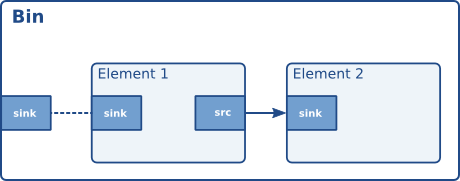
\includegraphics[width=1\textwidth]{figures/bin-element-ghost.png}
\end{figure}

\todo{Describe example figure + rtpbin + rtppay/depay}


\todo{Compare gstreamer with custom impl.}






\subsection{Publisher \& Subscriber}
\textbf{This is just notes.}
Describe given the nature of the stream, that publisher/subscriber most react on incoming data, and else do nothing until a new packet arrives.

This is similar to graphical interfaces, where the input is key press or clicks. This is event driven meaning a callback is invoked when an event is happening.
The subscriber should listen for the following events:
\begin{itemize}
	\item Incoming data packet from the producer
	\item Incoming metadata packet from the producer
	\item Periodically when metadata must be sent
\end{itemize}
\todo{Call "periodically event" for "temporal event"?}

The publisher should listen for the following events:
\begin{itemize}
	\item Incoming packet on stream
	\item Incoming metadata packet on stream
	\item Periodically when metadata must be sent.
\end{itemize}

alternative to event is polling, where the subscriber/publisher polls for data. This would be very CPU consuming and not utilize the functionality provided by the kernel.


\section{Stream Topology}

Master vs. nomaster
Cost of wellknown information(Profile + address, port) at all ends.
Describe how streams are put into sessions(RFC about semantics and taxonomics, pros and cons)

